\documentclass{beamer}
\usetheme{Madrid}
\usecolortheme{whale}

\usepackage{appendixnumberbeamer}
\usepackage{multimedia}
\usepackage{braket}
\usepackage{array}
\definecolor{mypurple}{RGB}{185,0,185}
\definecolor{mygreen}{RGB}{0,140,0}

\newcommand{\abs}[1]{\left\lvert #1 \right\rvert}
\graphicspath{ {Graphics/}  }
\setbeamerfont{caption}{size=\scriptsize}

\title[Ba-Yb Quantum Computing]{Mixed Species Ion Chains for Scalable Quantum Computation}
\subtitle{Exploring Using Barium Ions to Sympathetically Cool a Ytterbium Ion Quantum Computer}
\author[J. Wright]{John Wright}
\institute[UW] {
	Department of Physics \\
	University of Washington
}
\date[February 2015]{February 27, 2015}

\begin{document}

\begin{frame}[plain]
\titlepage
\end{frame}

\begin{frame}{Quantum Computing}
\begin{itemize}
	\item Shor's algorithm factors large integers for cryptology
	\item Grover's algorithm searches databases for specific elements
	\item Physical quantum phenomena are simulated in linear space
\end{itemize}
\vfill
\begin{columns}[c]
	\column{0.4\textwidth}
	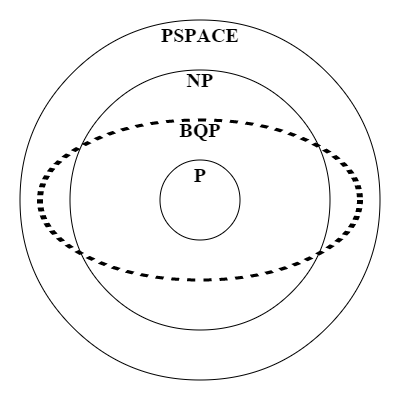
\includegraphics[width=0.9\textwidth]{BQP_complexity_class_diagram}
	\column{0.6\textwidth}
	\begin{itemize}
		\item P - polynomial time on a classical computer
		\item NP - polynomial time on a nondeterministic computer
		\item PSPACE - polynomial space on a classical computer
		\item BQP - bounded error polynomial time on a quantum computer
	\end{itemize}
\end{columns}
\end{frame}

\begin{frame}{Universal Set of Quantum Gates}
	\centerline{$
	H = \frac{1}{\sqrt{2}} \left(
		\begin{array}{cc} 1 & 1 \\ 1 & -1 \end{array}
	\right)$
	\hfill
	$T = \left(
		\begin{array}{cc} 1 & 0 \\ 0 & e^{i\pi/4} \end{array}
	\right)$
	\hfill
	$CNOT = \left(
		\begin{array}{cccc} 
			1 & 0 & 0 & 0 \\
			0 & 1 & 0 & 0 \\
			0 & 0 & 0 & 1 \\  
			0 & 0 & 1 & 0
		\end{array}
	\right)
	$}
\end{frame}

\begin{frame}{Bloch Sphere}
	\centerline{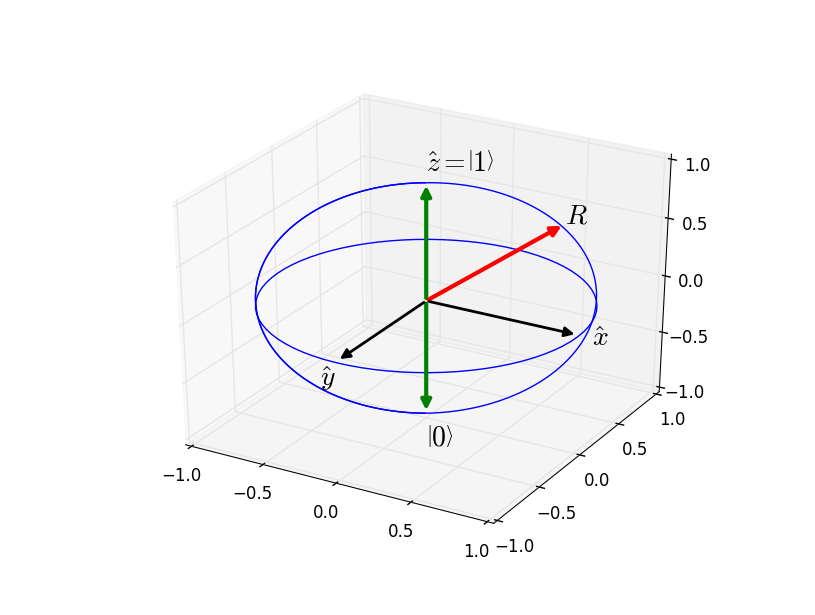
\includegraphics[width=0.6\textwidth]{Bloch_Sphere}}
	\vfill
\centerline{$\ket{\Psi} = \cos( \frac{\theta}{2} ) \ket{0} + \sin( \frac{\theta}{2} ) e^{i \phi} \ket{1}$}
\centerline{$\ket{\Psi} \sim R = \sin(\theta) \cos(\phi)\hat{x} + \sin(\theta) \sin(\phi)\hat{y} + \cos(\theta)\hat{z}$}
\end{frame}
	
\begin{frame}{Hadamard and T Gates}
	\centerline{Hadamard and T gates can be achieved with near resonant fields}
	\centerline{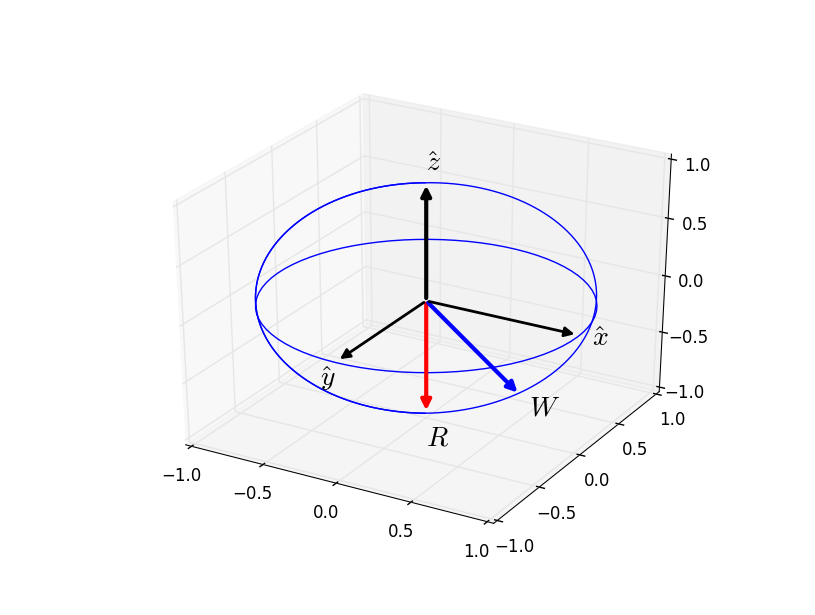
\includegraphics[width=0.6\textwidth]{Bloch_Sphere_W}}
	\centerline{$\dot{R} = R \times W$}
	\centerline{$W \equiv \Omega \hat{x} + \delta \hat{z}$}
\centerline{$\Omega$ = Rabi frequency \;\; $\delta$ = Frequency detuning from resonance}
\end{frame}

\begin{frame}{Ion Trapping}
	\centerline{CNOT gate requires use of ions' motional states}
	\centerline{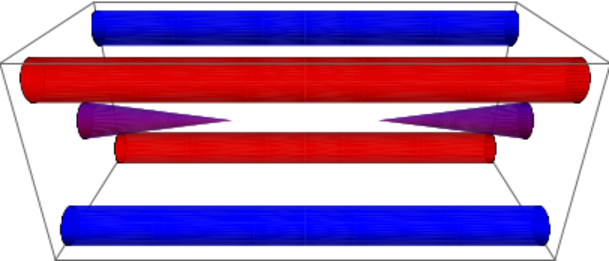
\includegraphics[width=0.7\textwidth]{PaulTrap}}
	\centerline{\colorbox{red}{\begin{minipage}{2cm}\end{minipage}} RF \;\; \colorbox{blue}{\begin{minipage}{2cm}\end{minipage}} GND \;\; \colorbox{mypurple}{\begin{minipage}{2cm}\end{minipage}} DC}
	\vfill
	\centerline{$\phi_\mathrm{dc} = \kappa_\mathrm{dc} V_\mathrm{dc} \left( z^2 - \frac{1}{2} \left( x^2 + y^2 \right) \right)$}
	\centerline{$\phi_\mathrm{rf} = \kappa_\mathrm{rf} V_\mathrm{rf} \cos( \Omega t ) \left( x^2 - y^2 \right)$}
	\vfill
	\centerline{$V_\mathrm{trap} = \frac{1}{2} m \omega_x^2 x^2 + \frac{1}{2} m \omega_y^2 y^2 + \frac{1}{2} m \omega_z^2 z^2$}
\end{frame}

\begin{frame}{Trapped Ion Normal Modes}
	\centerline{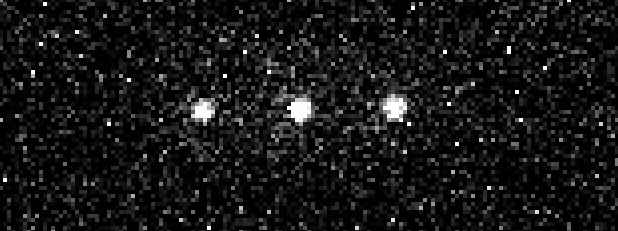
\includegraphics[width=0.5\textwidth]{ThreeIons}}
	\vfill
	\centerline{$V = V_\mathrm{trap} + \frac{1}{2}\sum\limits_{i \ne j}^N \frac{e^2}{4\pi\epsilon_0 \left| \vec{x}_i - \vec{x}_j \right|}$}
	\centerline{$\ddot{\xi}_{a,i} + \frac{1}{m} \sum\limits_{i=1}^{3N} \left( \frac{\partial}{\partial x_i}\frac{\partial}{\partial x_j} V \right) \xi_{a,j} = 0$}
	\centerline{$\xi_{a,i} = e_{a,i} e^{i \omega_a t}$}
\end{frame}

\begin{frame}{M\o{}lmer-S\o{}rensen Gates}
\centerline{CNOT gate can be achieved with a M\o{}lmer-S\o{}rensen gate}
\centerline{and single qubit operations}
\begin{columns}[c]
	\column{0.4\textwidth}
	\centerline{$\Omega_{MS} = \frac{\Omega^2 \eta^2}{ \nu - \delta }$} 
	\hfill \break
	\centerline{$\Omega$ = Rabi frequency}
	\centerline{$\eta = \sqrt{ \frac{\hbar}{2 m \nu} } k$} 
	\hfill \break
	\centerline{Require $\eta^2 \bar{n} \ll 1$}
	\column{0.6\textwidth}
	\centerline{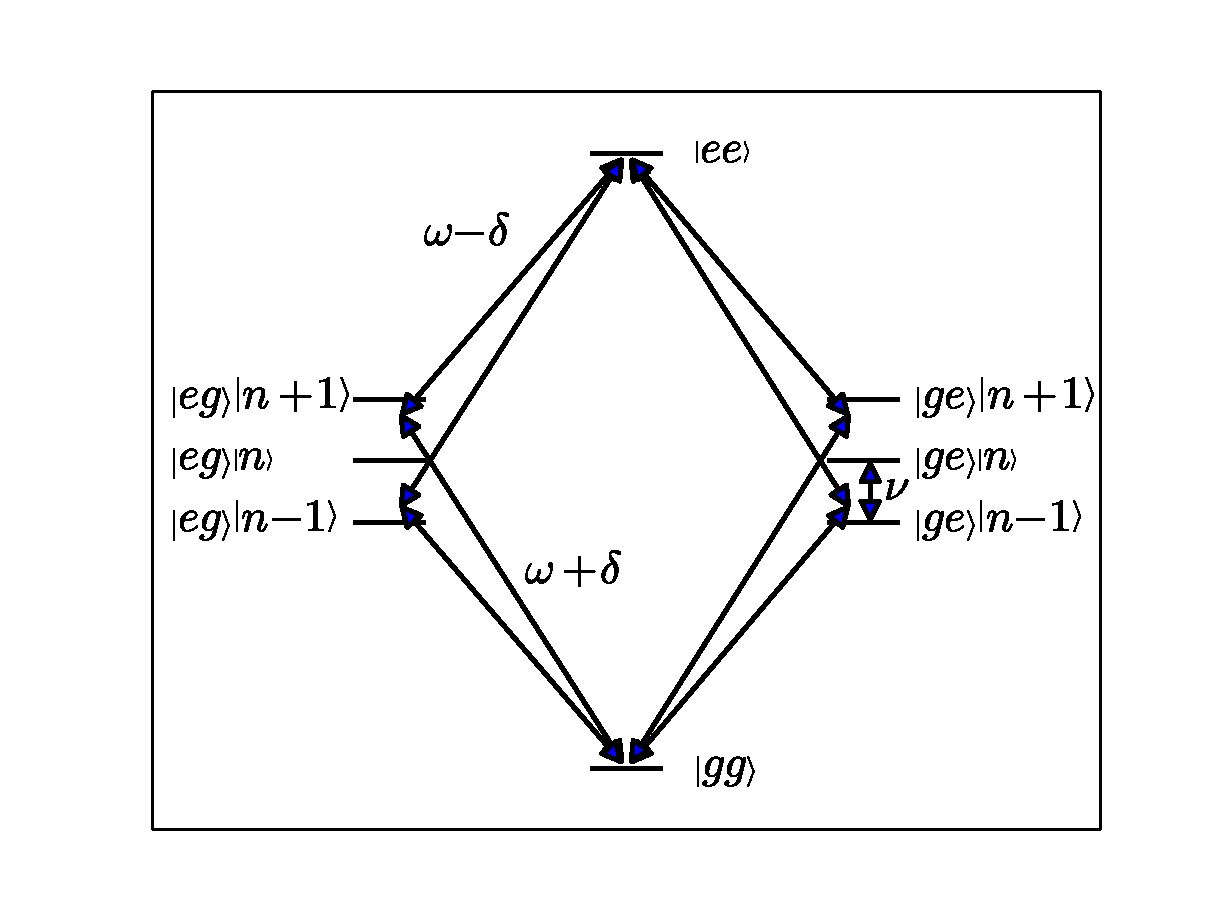
\includegraphics[height=0.7\textheight]{MolmerSorensen}}
\end{columns}
\end{frame}

\begin{frame}{Ion Trap Scaling}
	\centerline{\Large We need more ions}
	\begin{itemize}
		\item Most entangled ions is 14
		\item Error rates of $\approx$ 10$^{-4}$
		\item Error correction requires 10 to 100 times more ions
	\end{itemize}
	\vfill
	\centerline{\Large Getting more ions is hard}
	\begin{itemize}
		\item 3 motional modes per ion that decrease fidelity
		\item Modes get closer together in frequency
		\item Addressing ions separately and keeping them cold becomes increasingly hard
	\end{itemize}
\let\thefootnote\relax\footnote[frame]{T.Monz, et al, Phys. Rev. Lett., 106:130506, Mar 2011.}
\let\thefootnote\relax\footnote[frame]{K.R.Brown, et al, Phys. Rev. A, 84:030303, Sep 2011.}
\end{frame}

\begin{frame}{MUSIQC}
\textbf{Modular Universal Scalable Ion-Trap Quantum Computer Project}
\begin{itemize}
	\item Entangling ions in separate modular systems
	\item Microfabricated trap designs with many dc control voltages
	\item Separating tasks to different ion species to avoid crosstalk
\end{itemize}
\vfill
\centerline{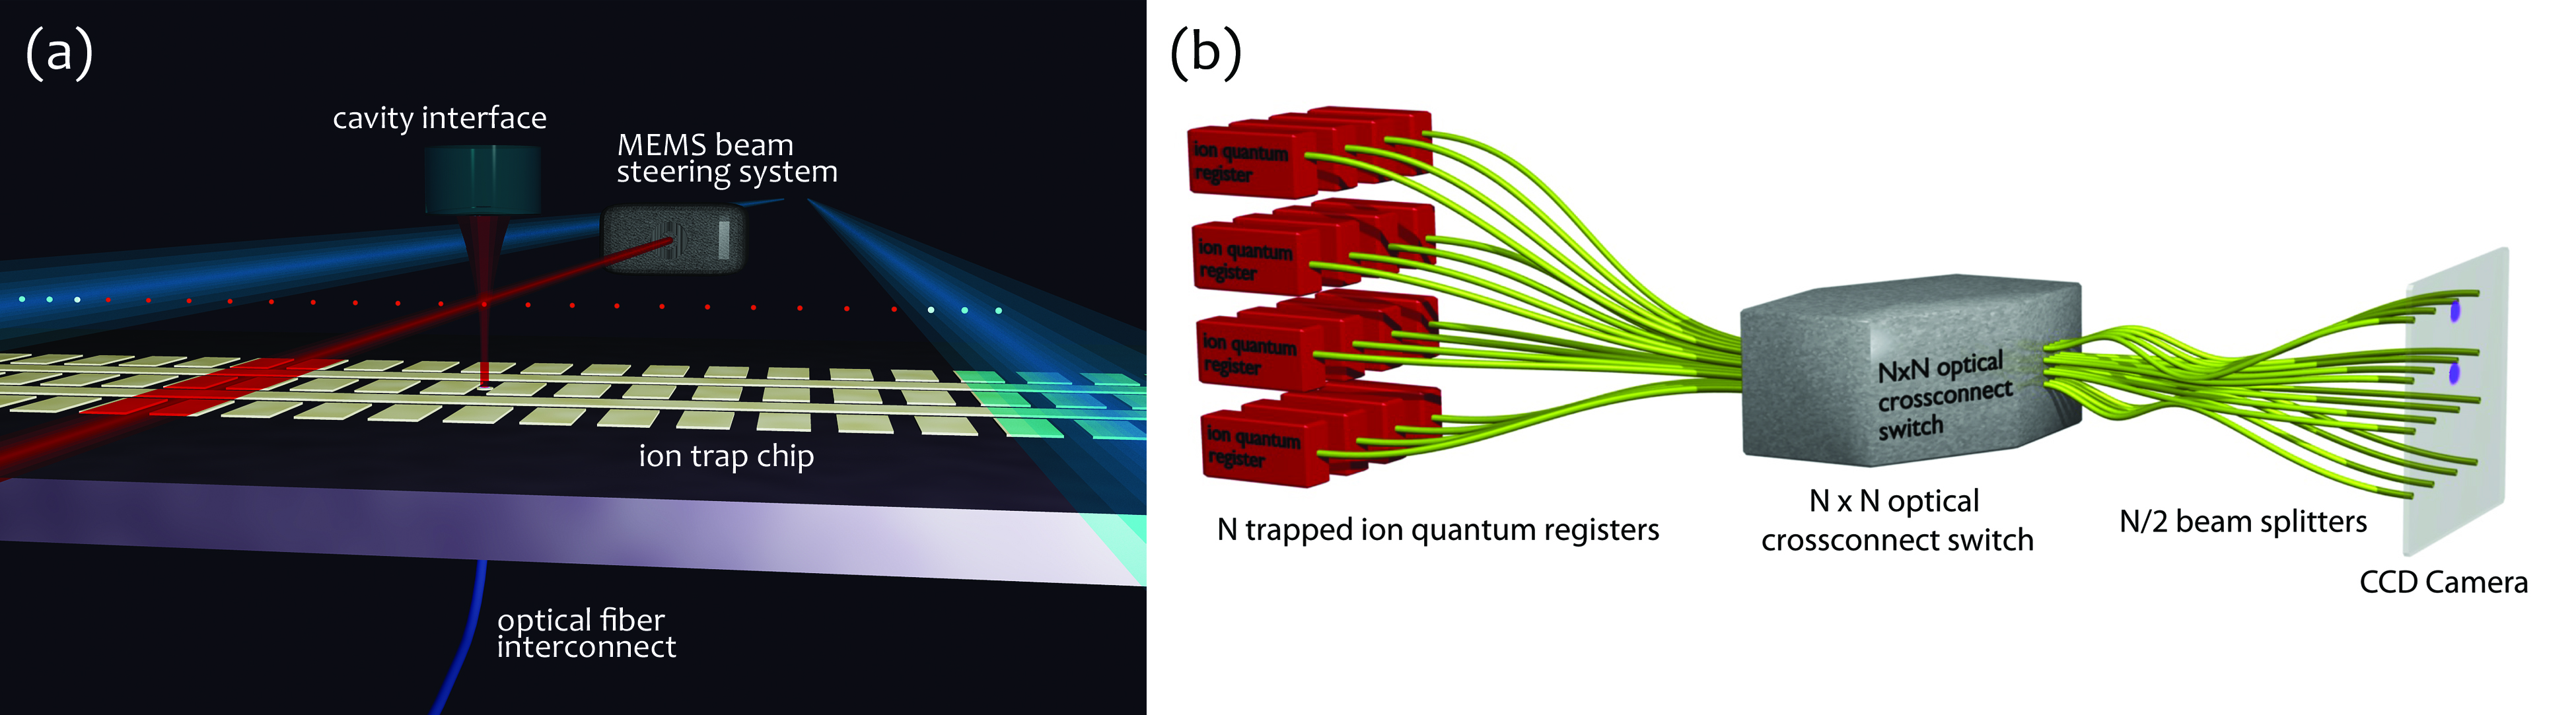
\includegraphics[height=0.38\textheight]{MUSIQC-plan}}
\let\thefootnote\relax\footnote[frame]{C.Monroe, et al, 2012, arXiv:1208.0391}
\end{frame}

\begin{frame}{Remote Ion-Ion Entanglement}
	\centerline{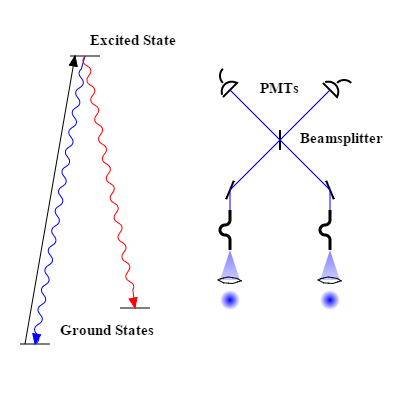
\includegraphics[width=0.5\textwidth]{remote-entanglement}}
	\centerline{$\ket{\Psi} = \bigotimes_{i=A,B} \frac{1}{\sqrt{2}} \left( \ket{H}_{i}\ket{\uparrow}_{i} + \ket{V}_{i}\ket{\downarrow}_{i} \right)$}
	\centerline{$\ket{\Psi} = \frac{1}{\sqrt{2}} \left( \ket{\uparrow}_A \ket{\downarrow}_B - \ket{\downarrow}_A \ket{\uparrow}_B \right)$}
\end{frame}

\begin{frame}{Surface Ion Traps}
	\centerline{\Large Sandia National Labs HOA Trap}
	\centerline{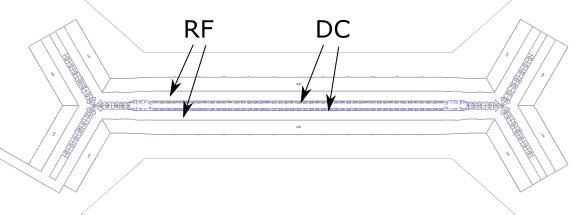
\includegraphics[width=0.9\textwidth]{HOA}}
\end{frame}

\begin{frame}{Boundary Element Method}
	\begin{table}\begin{tabular}{ccc}
		\centering
		& Induced Surface Charges & \\
		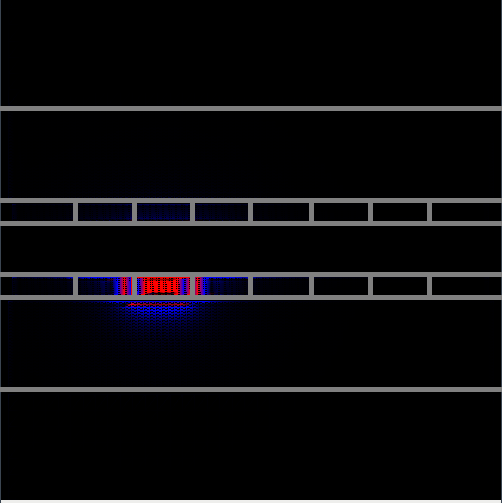
\includegraphics[width=0.3\textwidth]{dc_5} &
		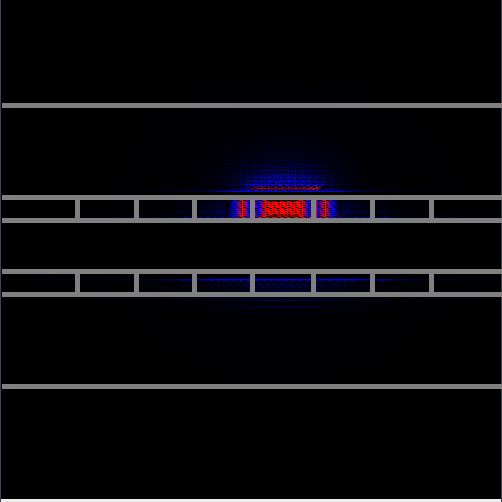
\includegraphics[width=0.3\textwidth]{dc_10} &
		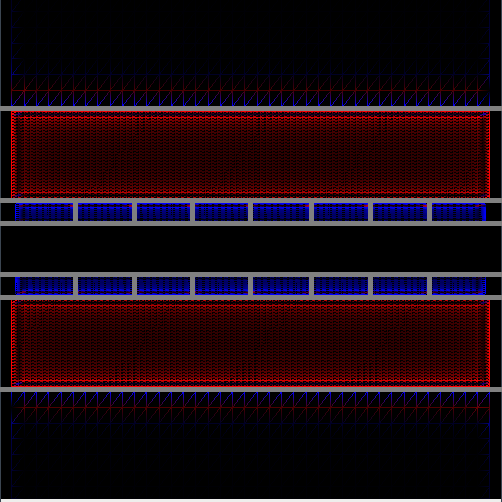
\includegraphics[width=0.3\textwidth]{rf_rails} \\

		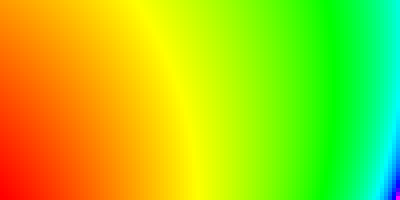
\includegraphics[width=0.3\textwidth]{yz_5} &
		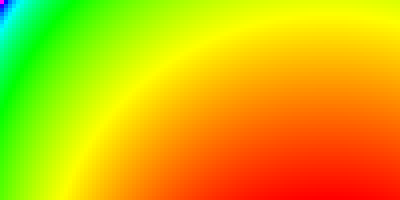
\includegraphics[width=0.3\textwidth]{yz_10} &
		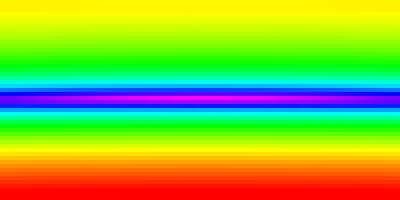
\includegraphics[width=0.3\textwidth]{yz_rf} \\
		& Potential in Trap Center &
	\end{tabular}\end{table}
\end{frame}

\begin{frame}{Trapping Solutions}
	\begin{table}\begin{tabular}{cc}
		\centering
		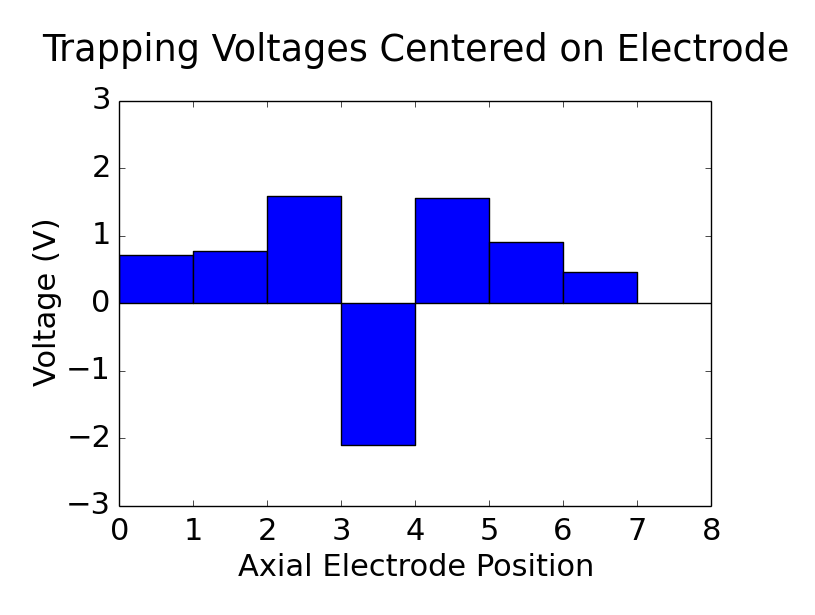
\includegraphics[width=0.4\textwidth]{center_trap} &
		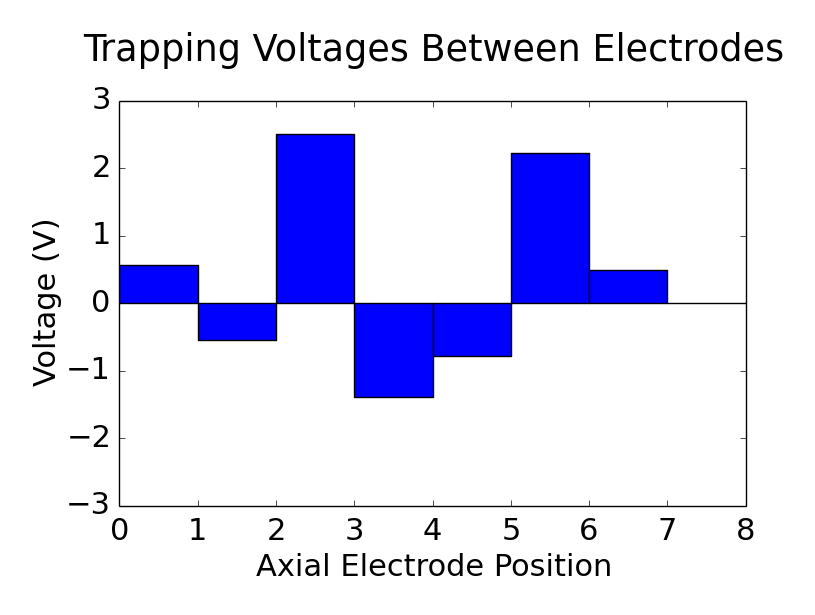
\includegraphics[width=0.4\textwidth]{inbetween_trap}  \\
		
		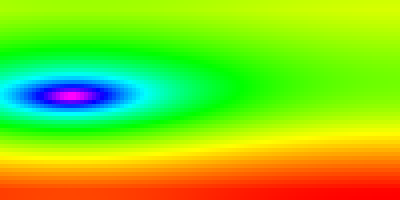
\includegraphics[width=0.4\textwidth]{yz_all_left} &
		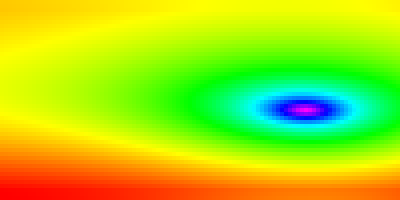
\includegraphics[width=0.4\textwidth]{yz_all}
	\end{tabular}\end{table}
\end{frame}

\begin{frame}{DAC System for DC Control}
	\centering
	\begin{itemize}
		\item 3 AD5372 DAC chips with 32 individually controllable output voltages
		\item Update rates up to 2~MHz via 50~MHz serial interface
		\item Custom FPGA system receives voltages via UDP and buffers updates to saturate DAC interface
	\end{itemize}
	\vfill
	\centerline{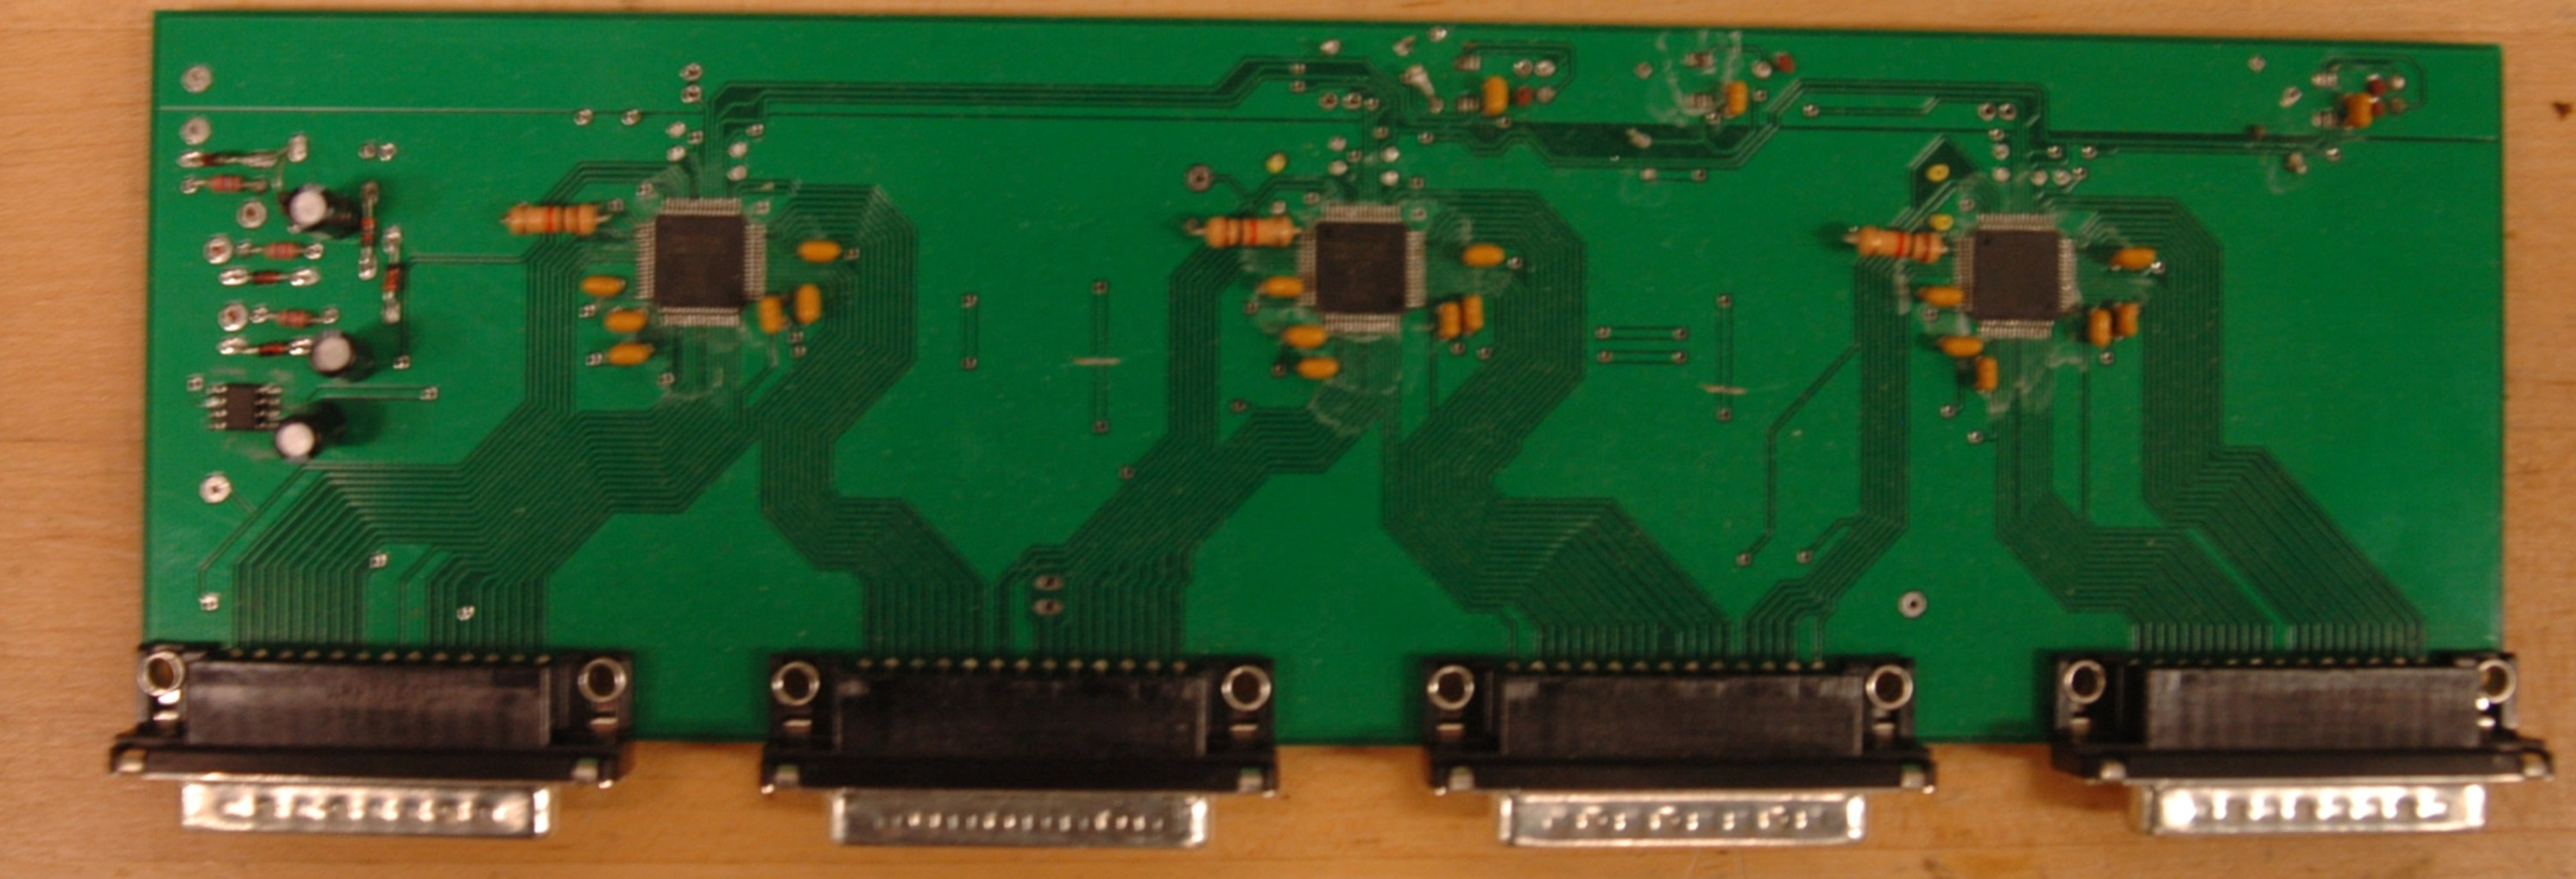
\includegraphics[width=0.8\textwidth]{DAC_board}}
\end{frame}

\begin{frame}{Surface Ion Traps}
	\centerline{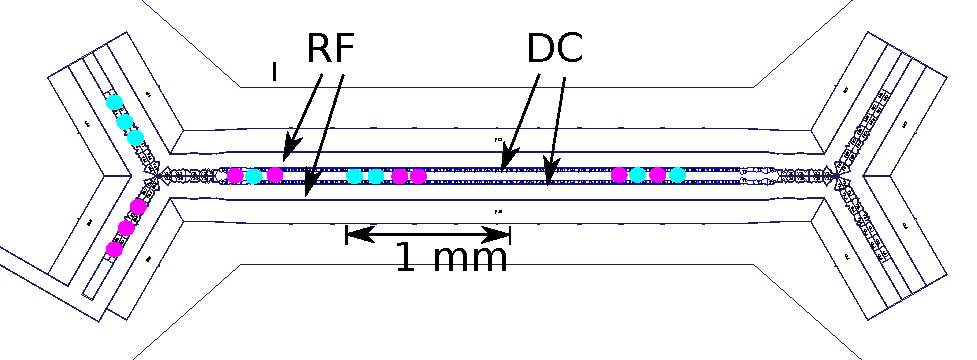
\includegraphics[width=0.9\textwidth]{HOA-ions}}
\end{frame}

\begin{frame}{Barium and Ytterbium Qubits}
\begin{columns}[T]
	\column{0.5\textwidth}
	\centerline{$^{138}$Ba$^+$ Zeeman Qubit}
	\begin{itemize}
		\item Coupled to 493~nm photons that transmit well in optical fiber
		\item Close in mass to ytterbium
		\hfill \break
		\item Sensitive to magnetic field noise
		\item Difficult to initialize and readout
	\end{itemize}
	\column{0.5\textwidth}
	\centerline{$^{171}$Yb$^+$ Hyperfine Qubit}
	\begin{itemize}
		\item Easy to initialize and readout
		\item First-order insensitive to magnetic field
		\item Coherence times of seconds without shielding
		\hfill \break
		\item Coupled to 369~nm photons that do not transmit well in optical fiber
	\end{itemize}
\let\thefootnote\relax\footnote[frame]{S.Olmschenk, Phys. Rev. A, 76:052314, Nov 2007.}
\end{columns}


\end{frame}

\begin{frame}{Ionizing Barium and Ytterbium}
	\centering
	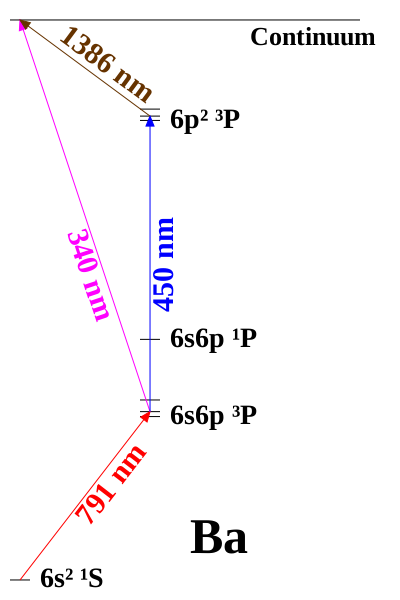
\includegraphics[width=0.4\textwidth]{neutral-Ba}
	\hfill
	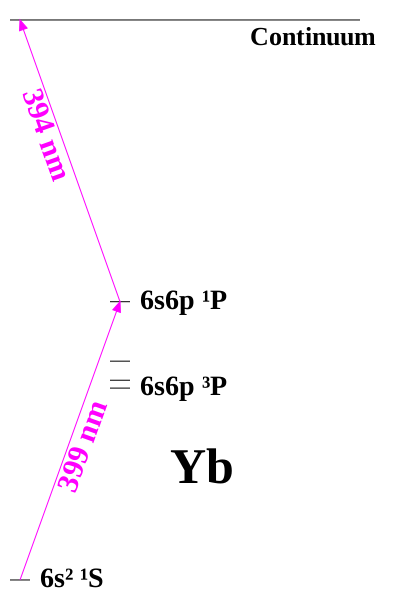
\includegraphics[width=0.4\textwidth]{neutral-Yb}
\end{frame}

\begin{frame}{Doppler Cooling Barium and Ytterbium}
	\centering
	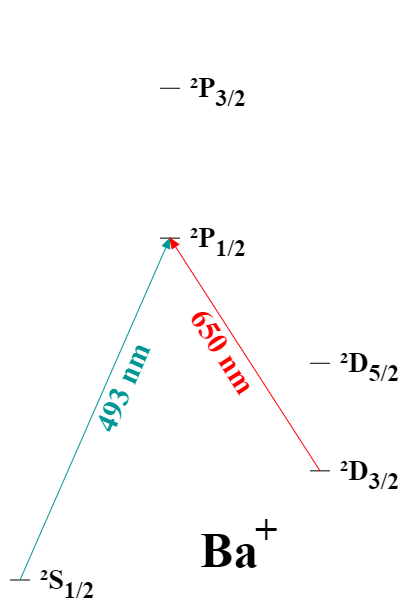
\includegraphics[width=0.4\textwidth]{ionized-Ba-cooling}
	\hfill
	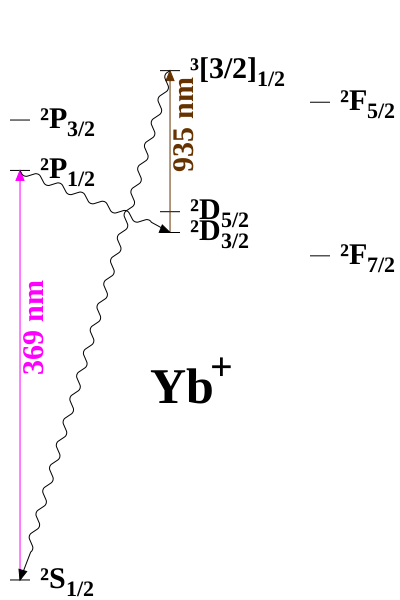
\includegraphics[width=0.4\textwidth]{ionized-Yb}
\end{frame}

\begin{frame}{Doppler Cooling}
	\centerline{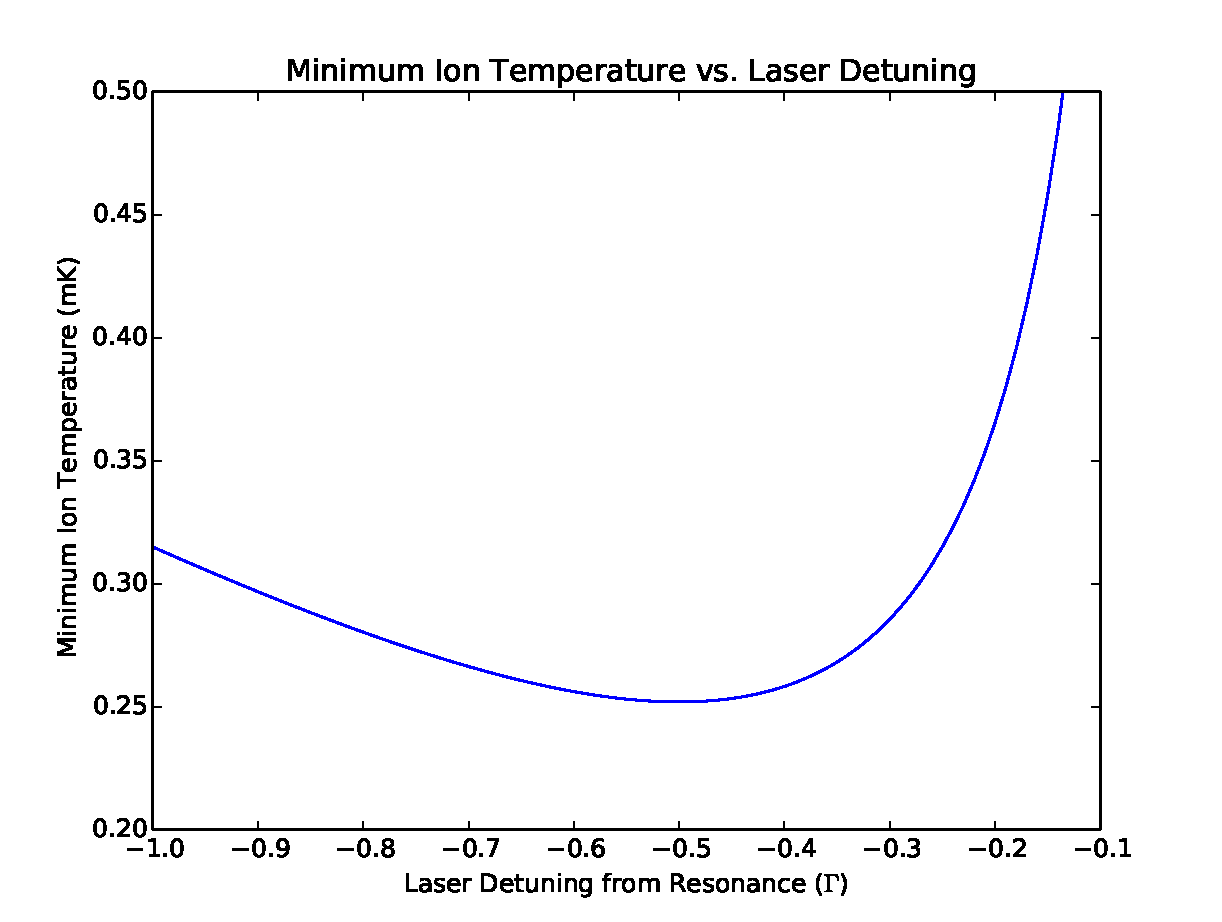
\includegraphics[width=0.6\textwidth]{DopplerCooling}}
	\centerline{$F_\mathrm{scatter}( v_{ion} ) = \hbar k R_\mathrm{scatter}( v_{ion} ) \approx F(  0) - \alpha v_{ion}$}
\end{frame}

\begin{frame}{1762~nm Transitions in Ba}
\begin{columns}[c]
	\column{0.5\textwidth}
	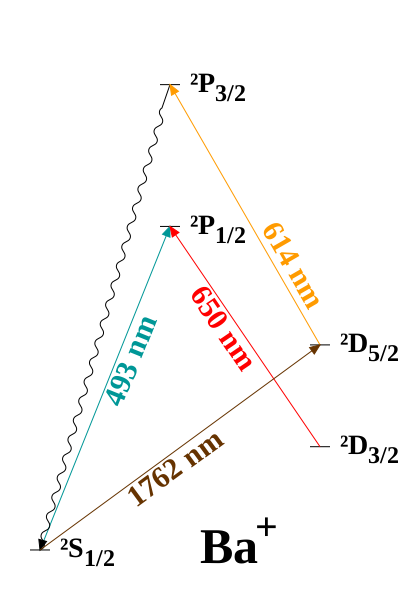
\includegraphics[width=0.9\textwidth]{ionized-Ba}
	\column{0.5\textwidth}
	\begin{itemize}
		\item Shutter cooling lasers
		\item Initialize ion in 6S$_{1/2}$
		\item Apply 1762~nm pulse
		\item Unshutter cooling lasers
		\item 5D$_{5/2}$  has 30~s lifetime and is outside of the cooling cycle
	\end{itemize}
	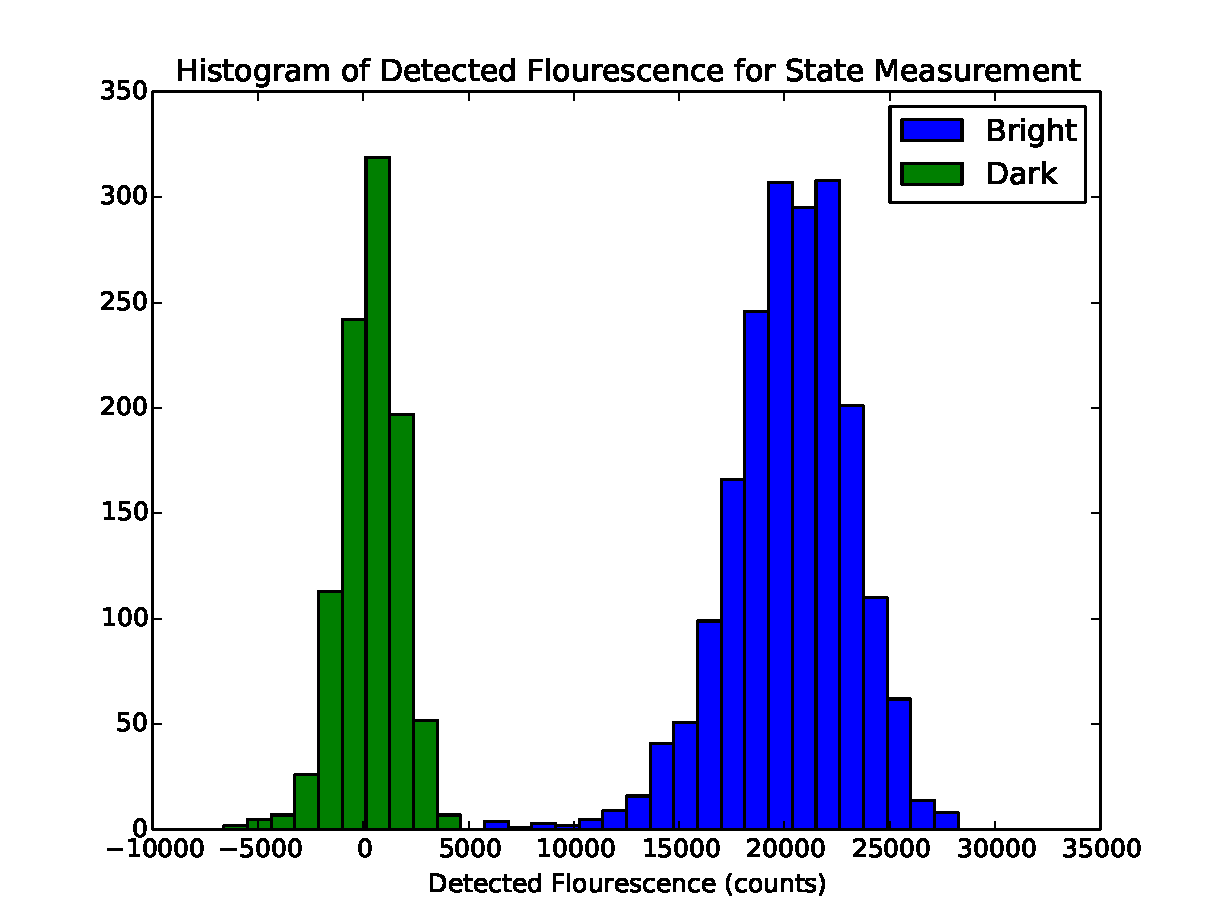
\includegraphics[width=0.9\textwidth]{StateMeasurement}
\end{columns}
\end{frame}

\begin{frame}{Rabi Flop Interference}
	\centerline{
		\includegraphics<1>[height=0.7\textheight]{HeatingRateT0Orange}
		\includegraphics<2>[height=0.7\textheight]{HeatingRateBoth}
	}
\visible<2->{\centerline{\colorbox{red}{\begin{minipage}{2cm}\end{minipage}} No Delay (26 $\pm$ 18~quanta) \;\; \colorbox{mygreen}{\begin{minipage}{2cm}\end{minipage}} 50~ms Delay (166 $\pm$ 15~quanta)}}
	\centerline{$P_\mathrm{shelve} = \sum\limits_{n=0}^{\infty} \frac{1}{\bar{n} + 1} \left( \frac{\bar{n}}{\bar{n}+1} \right)^n \sin^2\left( \Omega_0 (1 - \eta^2 n ) t \right)$}
\end{frame}

\begin{frame}{Heating Rate}
	\centerline{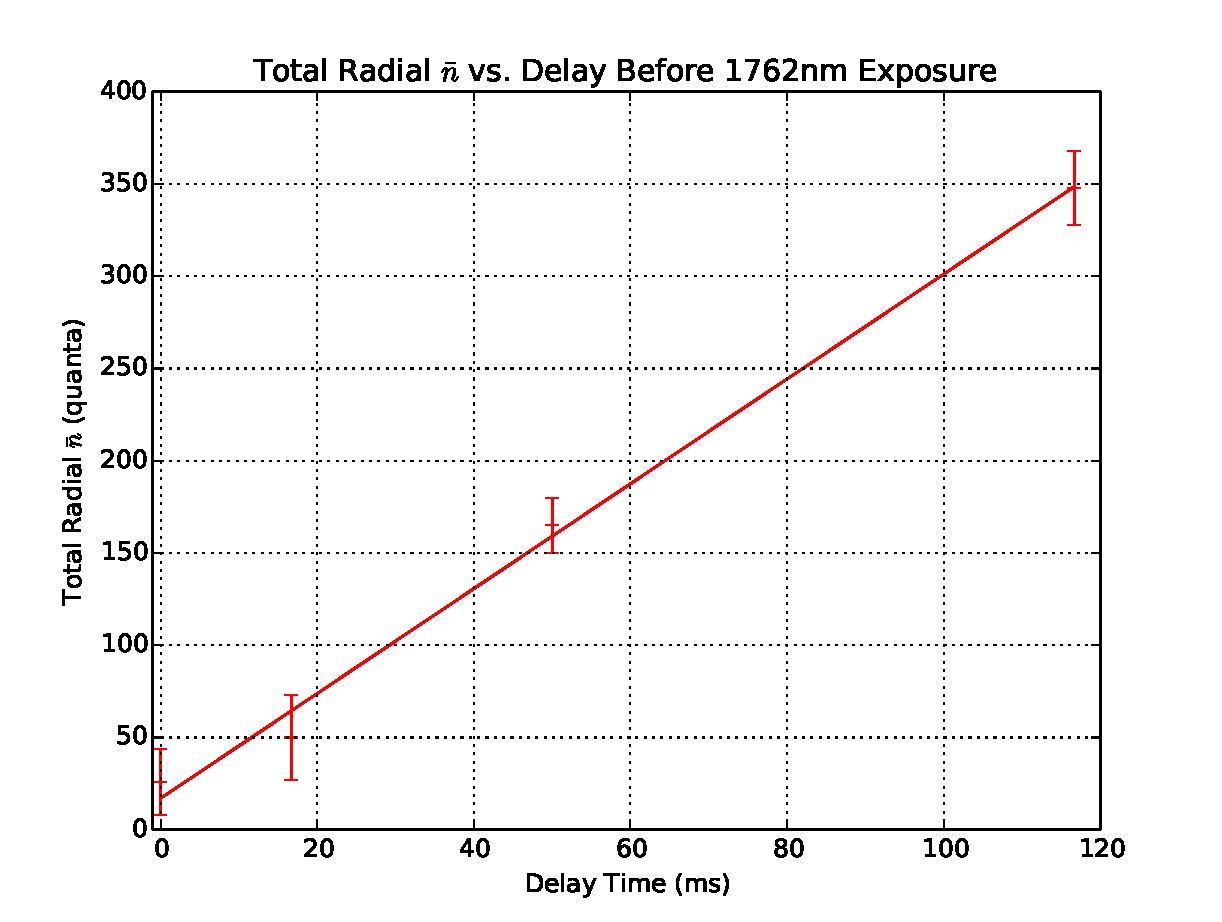
\includegraphics[width=0.8\textwidth]{HeatingRateNoise}}
	\centerline{Initial $\bar{n}$ = 17~quanta \; \;  Heating Rate = 2.84~quanta/ms}
\end{frame}

\begin{frame}{Mixed Species Chains}
	\centerline{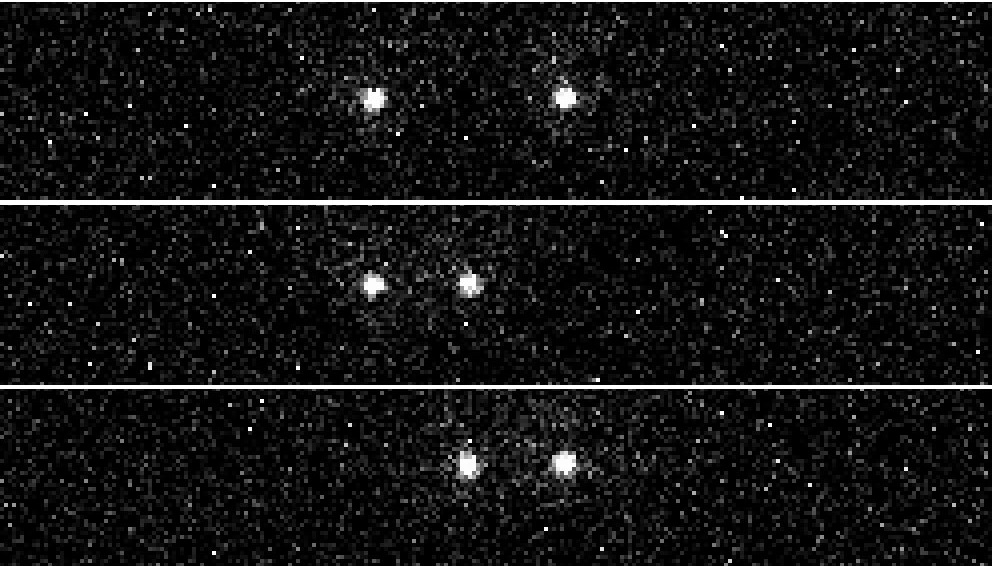
\includegraphics[width=0.5\textwidth]{BaYb}}
	\vfill
	\pause
	\centerline{$V = V_\mathrm{trap} + \frac{1}{2}\sum\limits_{i \ne j}^N \frac{e^2}{4\pi\epsilon_0 \left| \vec{x}_i - \vec{x}_j \right|}$}
	\centerline{$\ddot{\xi}_{a,i} + \sum\limits_{i=1}^{3N} \frac{1}{\sqrt{m_i m_j}} \left( \frac{\partial}{\partial x_i}\frac{\partial}{\partial x_j} V \right) \xi_{a,j} = 0$}
	\centerline{$\xi_{a,i} = e_{a,i} e^{i \omega_a t}$}
\end{frame}

\begin{frame}{Mixed Species Normal Modes}
	\centerline{\Large Ba-Ba-Yb-Yb Normal Modes}
	\centerline{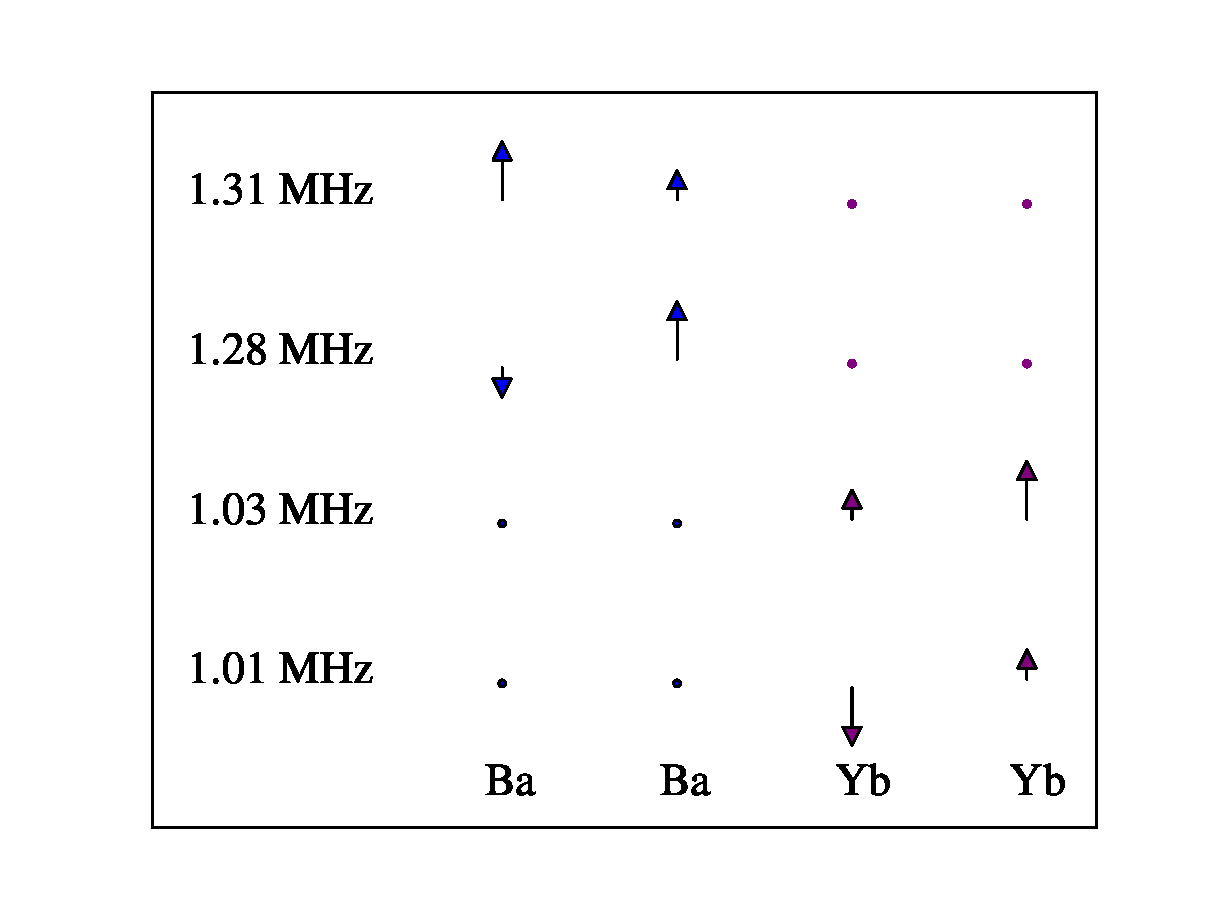
\includegraphics[width=0.7\textwidth]{BBYYNormalModes}}
	\centerline{Modes couple to one ion species 20 to 40 times more stongly than the other}
\end{frame}

\begin{frame}{1762~nm Frequency Scans}
	\centerline{Rabi frequency technique doesn't work for large chains}
	\centerline{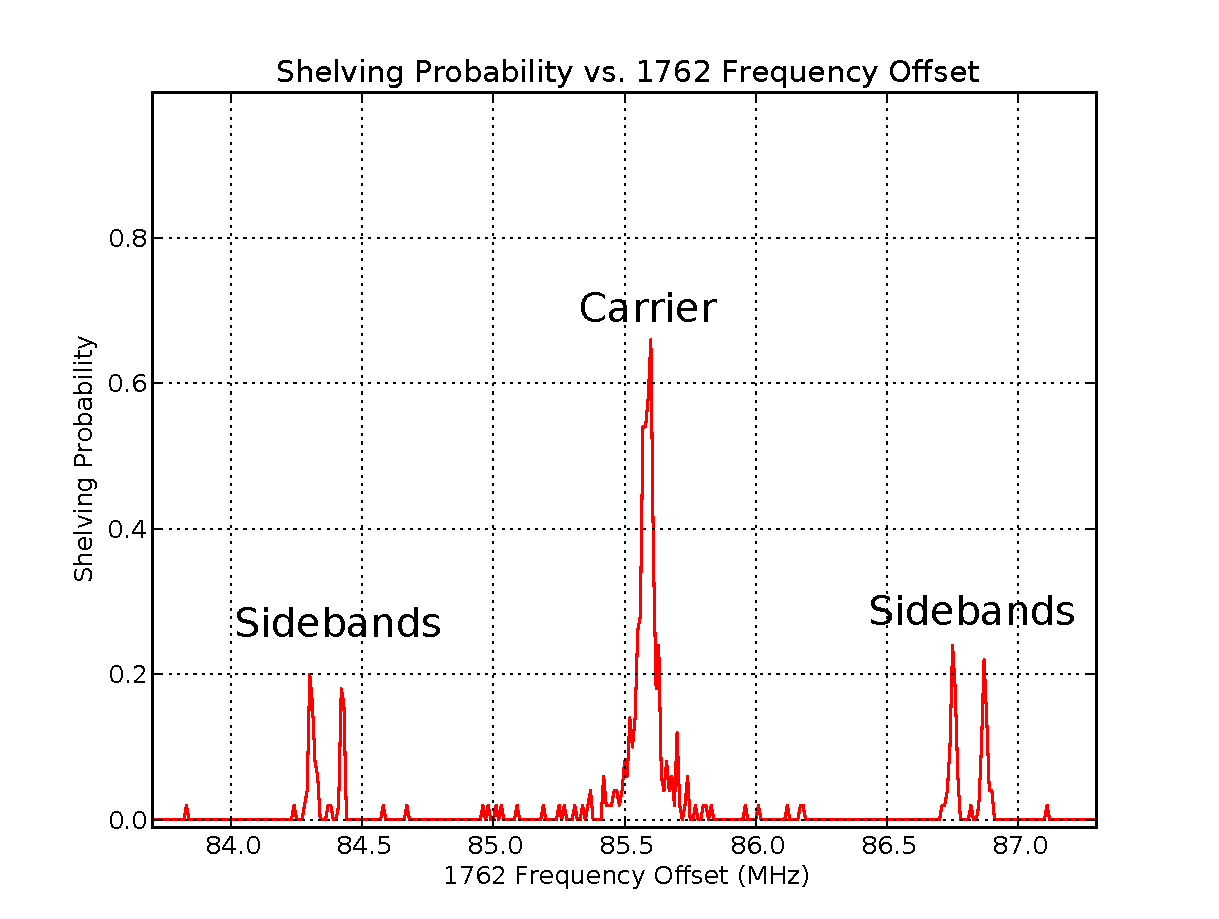
\includegraphics[width=0.75\textwidth]{FullScan}}
	\vfill
	\centerline{${\Large\bra{e_i}\bra{n_{a} \pm 1}} \; \widehat{E2} \; {\Large \ket{n_{a}}\ket{g_i}} \propto \sqrt{n_{a}} e_{a,i}$}
\end{frame}

\begin{frame}{Radial Mode Scans}
	\centerline{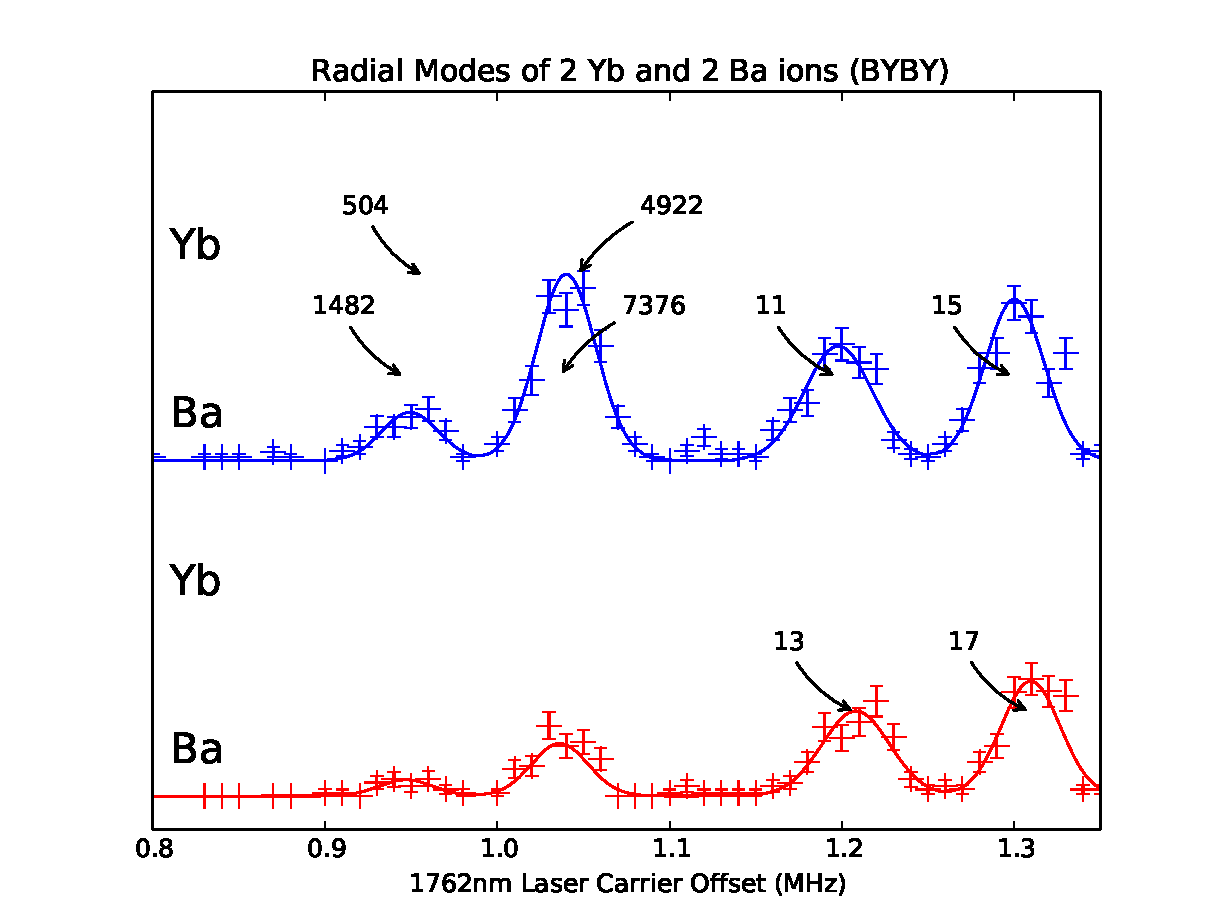
\includegraphics[width=0.9\textwidth]{RadialScanBYBY}}
\end{frame}

\begin{frame}{Radial Mode Scans}
	\centerline{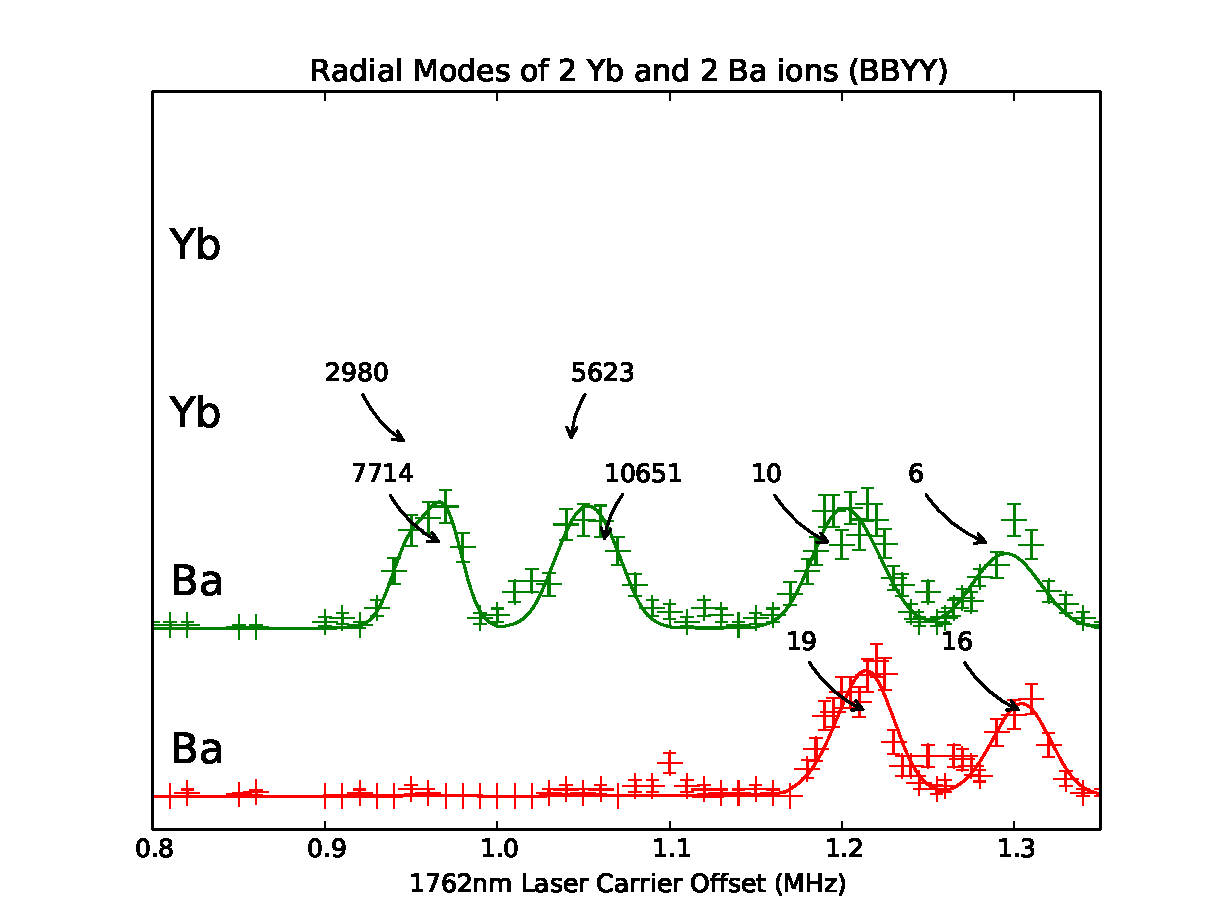
\includegraphics[width=0.9\textwidth]{RadialScanBBYY}}
\end{frame}

\begin{frame}{Radial Mode Scan Results}
	\centerline{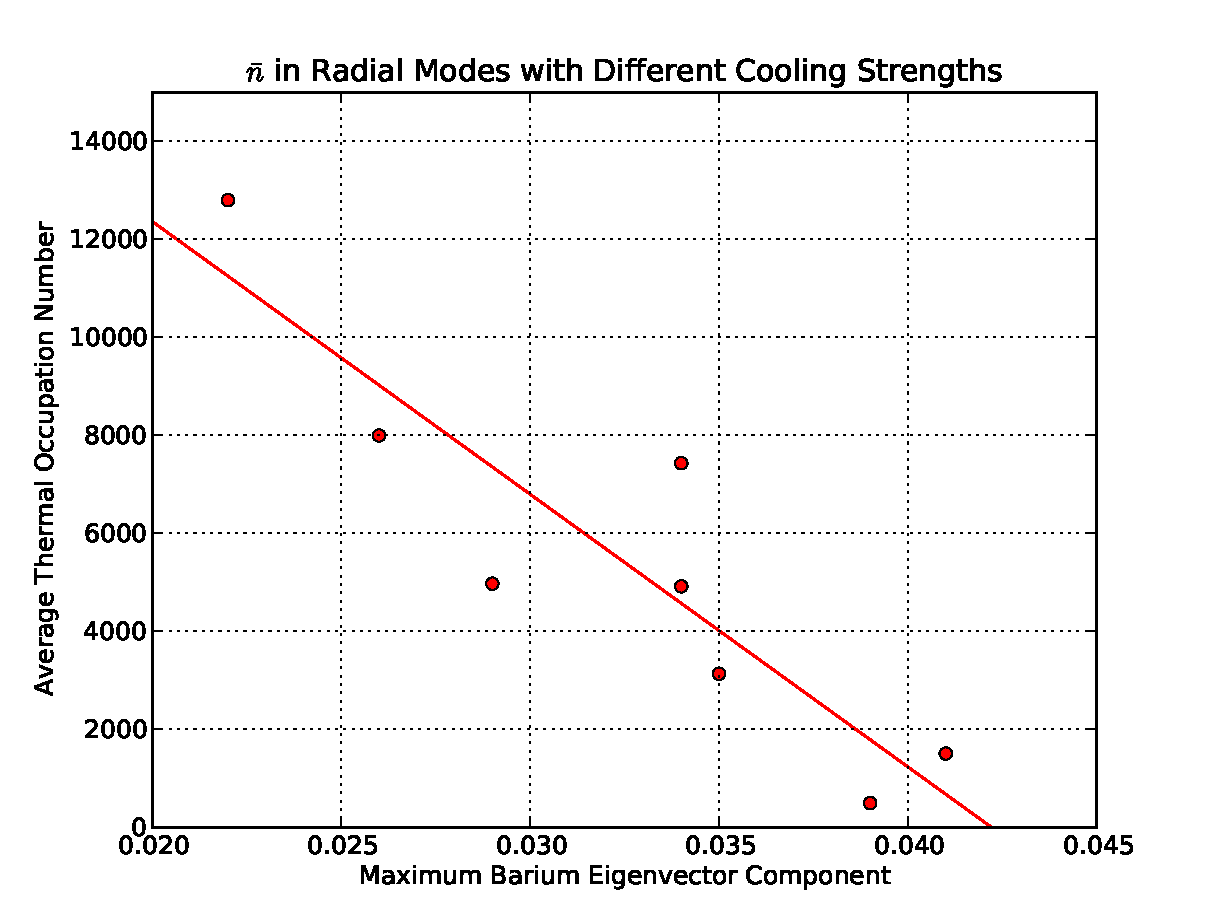
\includegraphics[width=0.8\textwidth]{RadialNBarEigenvectors}}
	\pause
	\centerline{Require $\eta^2 \bar{n} \ll 1$}
\end{frame}

\begin{frame}{Ion Species Reordering}
	\centerline{\Large Ion species reordering is also a temperature probe.}
	\centerline{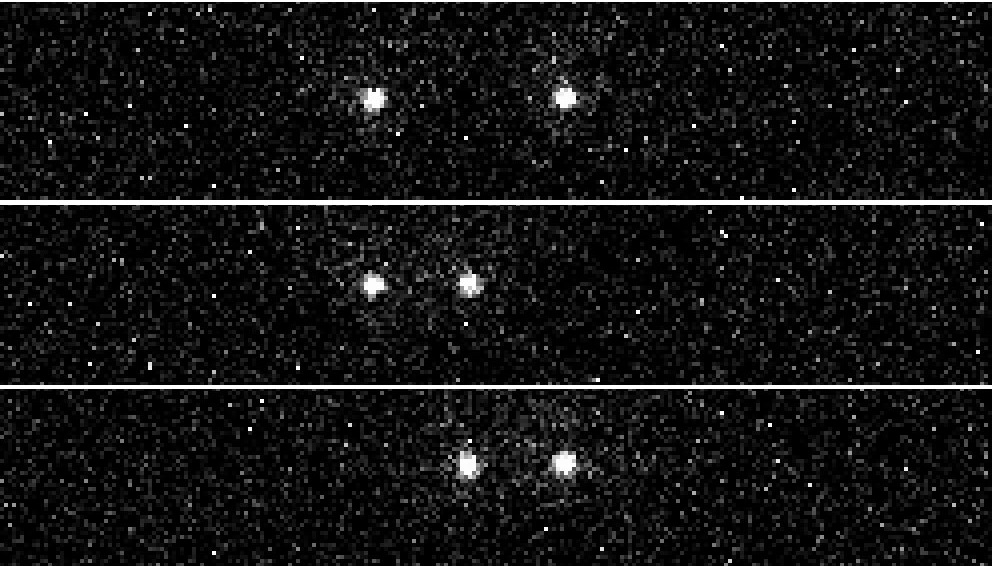
\includegraphics[width=0.5\textwidth]{BaYb}}
	\begin{itemize}
		\item Take CCD image of ion positions
		\item Shutter cooling lasers and delay to allow heating
		\item Unshutter cooling lasers and reimage ions
			\hfill \break
		\item Measurements take minutes instead of hours
		\item Provides average measurements of all motional modes
	\end{itemize}
\end{frame}

\begin{frame}{Ion Species Reordering}
	\centerline{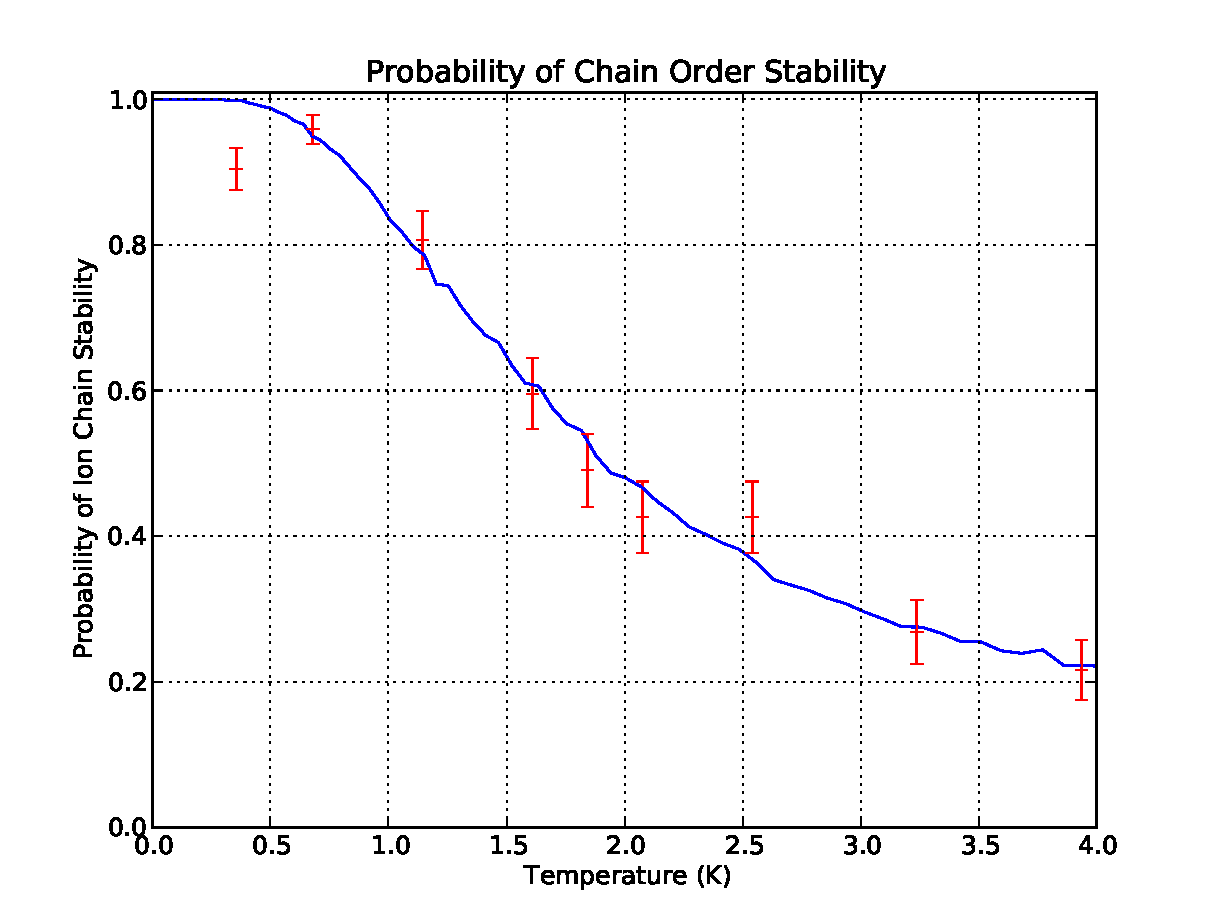
\includegraphics[width=0.8\textwidth]{Reordering81}}
	\centerline{\Large Chain of 7 barium and 1 ytterbium ion}
\end{frame}

\begin{frame}{Ion Reordering Simulations}
	\centerline{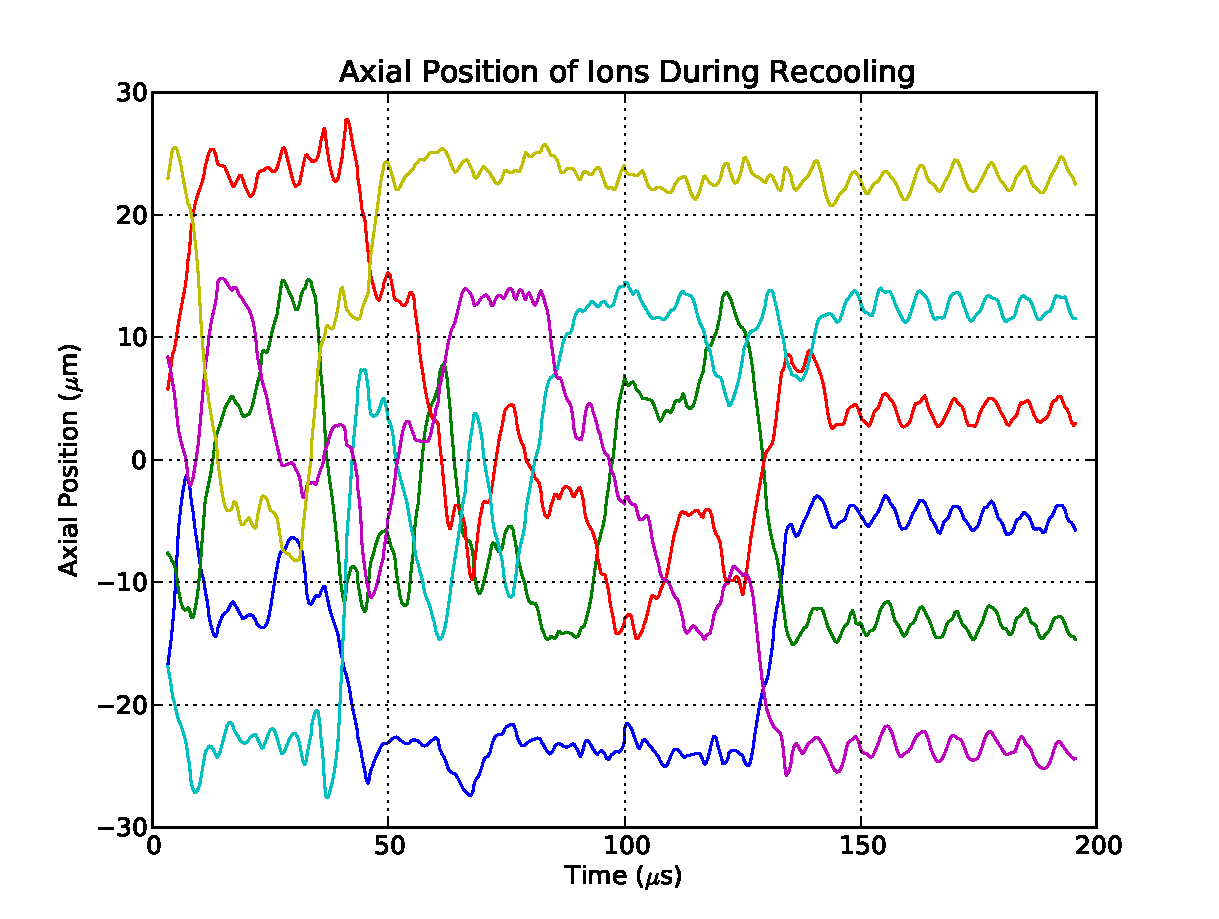
\includegraphics[width=0.8\textwidth]{ReorderingPositions}}
\end{frame}

\begin{frame}{Ion Species Reordering}
	\centerline{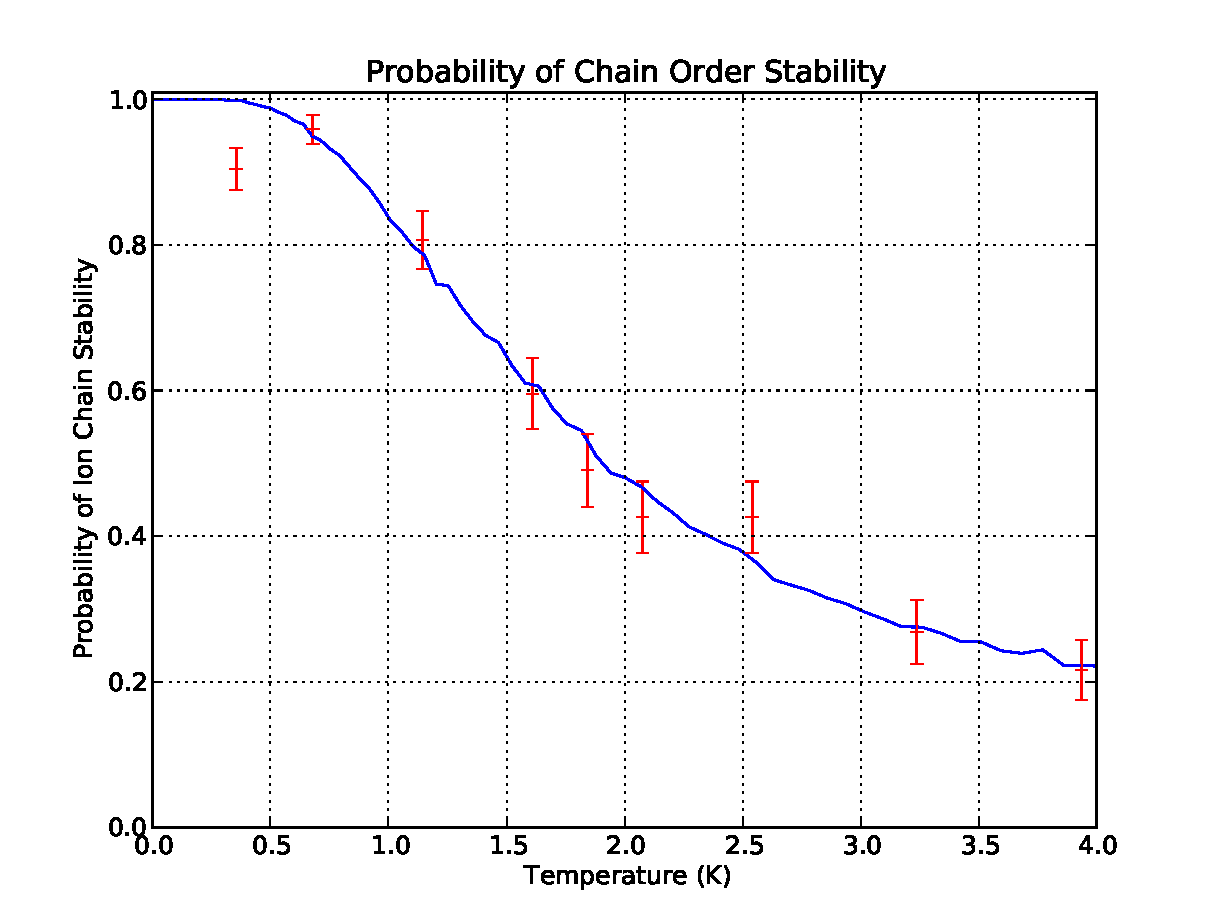
\includegraphics[width=0.8\textwidth]{Reordering81}}
	\centerline{T$_\mathrm{initial}$ = 0.221~K \;\; $\dot{T}$ = 0.44~K/s (7.19~quanta/ms)}
\end{frame}

\begin{frame}{Heating Rate and Temperature Summary}
	\begin{itemize}
		\item We are right on the border of keeping ytterbium ions usefully cold using only barium Doppler cooling
		\item We have developed tools and techniques to characterize the temperature and heating rate in mixed ion systems
		\item Surface traps will allow us to work with this system more easily and give us more trap degrees of freedom
		\item Need quantum operations to test
	\end{itemize}
\end{frame}

\begin{frame}{Zeeman Rabi Transitions}
\begin{columns}[c]
	\column{0.5\textwidth}
	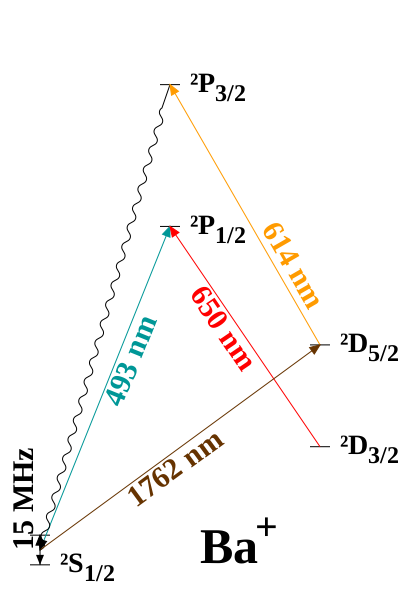
\includegraphics[width=0.9\textwidth]{ionized-Ba-zeeman}
	\column{0.5\textwidth}
	\begin{itemize}
		\item Shutter cooling lasers
		\item Initialize ion into individual Zeeman state
		\item Apply resonant Zeeman rf pulse
		\item Apply resonant 1762~nm $\pi$-pulse
		\item Unshutter cooling lasers
	\end{itemize}
\end{columns}
\end{frame}

\begin{frame}{Zeeman Rabi Flops}
	\centerline{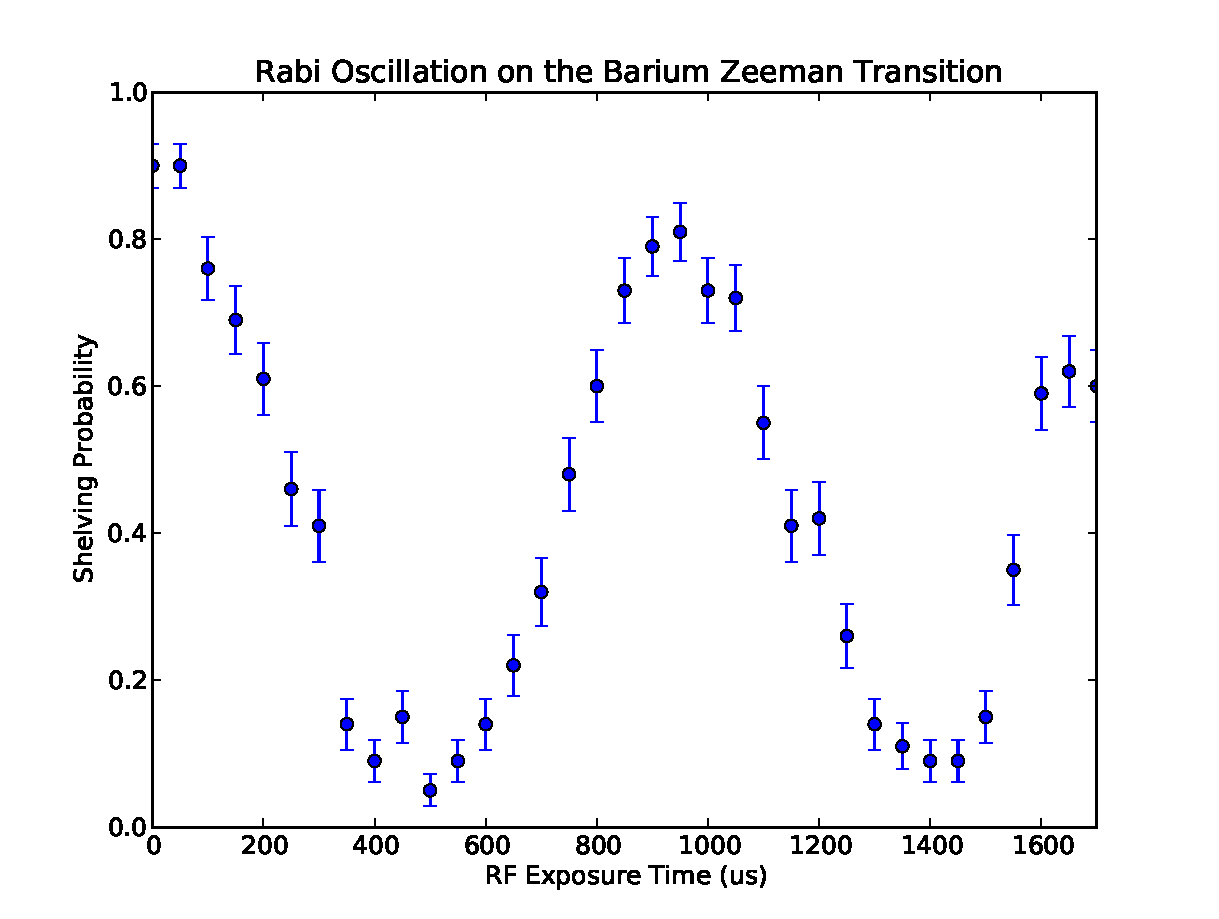
\includegraphics[width=0.8\textwidth]{ZeemanRabi}}
	\centerline{\Large $\lambda \approx$ 20 meters \;\; $\eta \approx$ 10$^{-9}$ \;\; $\Omega_{MS} = \frac{\Omega^2 \eta^2}{ \nu - \delta }$}
\end{frame}

\begin{frame}{Raman Transitions in Ba}
\begin{columns}[c]
	\column{0.5\textwidth}
	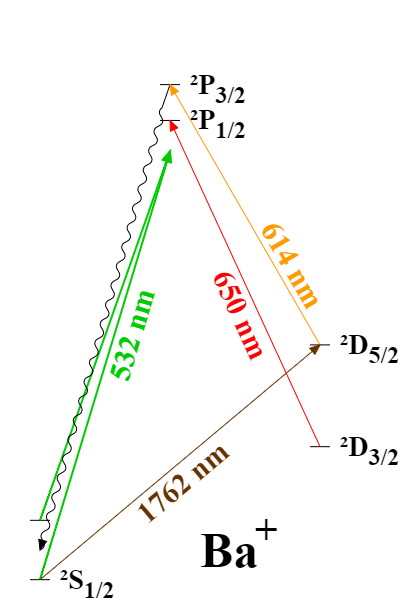
\includegraphics[width=0.9\textwidth]{ionized-Ba-raman}
	\column{0.5\textwidth}
	\centerline{$ \Omega = \frac{ \left| \mu \right|^2 \left| E \right|^2}{ \Delta }$}
	\centerline{Detuning $\Delta$ = 2$\pi$ $\times$ 44~THz}
	\hfill \break
	\begin{itemize}
		\item Optical transitions can be addressed onto single ions
		\item Lamb-Dicke parameter can be large ($\approx$ 0.05)
	\end{itemize}
\end{columns}
\end{frame}

\begin{frame}{Millennia Laser}
	\centerline{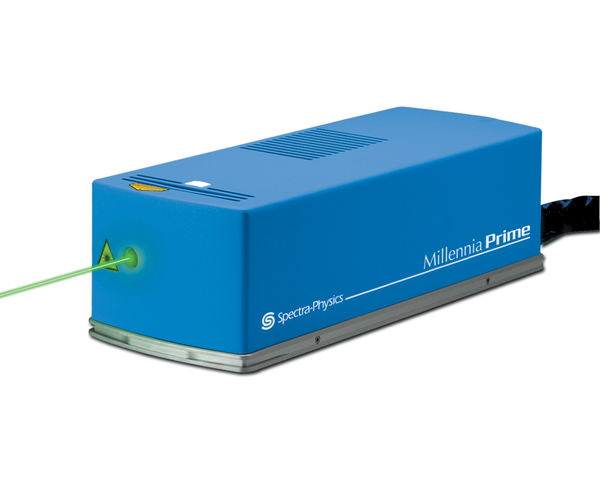
\includegraphics[width=0.6\textwidth]{Millennia}}
	\centerline{\Large Producing 500~mW of 532~nm light in 17~ps pulses}
\end{frame}

\begin{frame}{Raman Transitions}
	\centerline{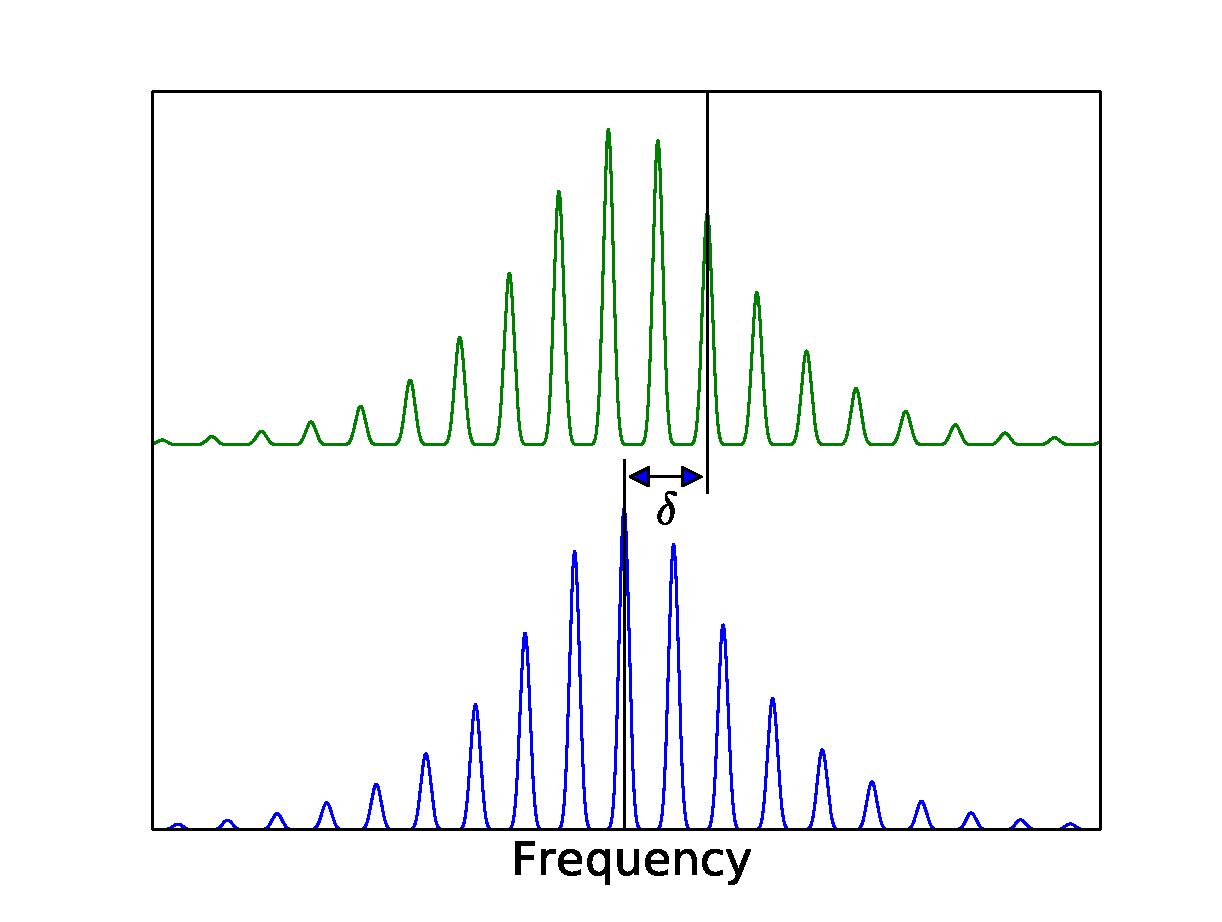
\includegraphics[width=0.8\textwidth]{Raman}}
	\centerline{Frequency comb teeth can be tuned to drive transitions}
\end{frame}

\section[]{Conclusions}
\begin{frame}{Conclusions}
\begin{itemize}
	\item Quantum computing with trapped ions is making rapid progress
	\item Surface ion traps enable us to have separate trapping regions in the same vacuum system and to reorganize ions of different species
	\item Using mixed species chains will allow longer quantum operations to be carried out by continuously cooling one ion species
	\item Together these technologies will help us scale the number of communicating ions to computationally useful numbers
\end{itemize}
\end{frame}

\begin{frame}{Thank You}
\centering
PI: Boris Blinov
\begin{block}{MUSIQC}
\begin{tabular*}{0.9\textwidth}{p{0.3\linewidth} p{0.3\linewidth} p{0.3\linewidth}}
Tomasz Sakrejda & Richard Graham & Zichao Zhou \\
\end{tabular*}
\end{block}

\begin{block}{Ion Trappers}
\begin{tabular*}{0.9\textwidth}{p{0.3\linewidth} p{0.3\linewidth} p{0.3\linewidth}}
Tom Noel & Carolyn Auchter & Chen-Kuan Chou \\
Matt Hoffman & Spencer Williams & Anupriya Jayakumar \\
Matt Bohman & Wen Lin Tan
\end{tabular*}
\end{block}

\begin{columns}
\begin{column}{0.5\textwidth}
	
\includegraphics[width=0.9\textwidth]{musiqc_logo}
\end{column}
\begin{column}{0.5\textwidth}
	
\includegraphics[width=0.9\textwidth]{iarpa}
\end{column}
\end{columns}
\end{frame}

\end{document}
